\documentclass[11pt]{article}
% /usr/local/texlive/2013/bin/x86_64-darwin/pdflatex 
\usepackage[T1]{fontenc}
\usepackage[utf8]{inputenc}
\usepackage[fleqn]{amsmath}
\usepackage{amssymb}
\usepackage{graphicx}
\usepackage{hyperref}
\usepackage{parskip}
\usepackage{tikz} 
\usepackage{wrapfig} 
\usepackage[letterpaper]{geometry}
\linespread{1.35}
\usepackage[font=small,labelfont=bf]{caption}
%\usepackage{cancel}

% körper und mengen
\newcommand{\setn}{\mathbb N}
\newcommand{\setr}{\mathbb R}
\newcommand{\setc}{\mathbb C}
\newcommand{\setk}{\mathbb K}

% reihe von #1 bis unendlich über #2
\newcommand{\reihe}[2]{\sum\limits_{#1}^{\infty}{#2}}
% summe von #1 bis #2 über #3
\newcommand{\summe}[3]{\sum\limits_{#1}^{#2}{#3}}
% integral von #1 bis #2 über #3 nach #4
\newcommand{\integrald}[4]{\int\limits_{#1}^{#2}{#3 \; \mathrm d#4}}
% integral von #1 bis #2 über #3 (d/dx muss dann selbst angegeben werden)
\newcommand{\integral}[3]{\int\limits_{#1}^{#2}{#3}}
% integralberechnung von #1 bis #2 über 3
\newcommand{\integralv}[3]{\left[ #3 \right]_{#1}^{#2}}
% betrag mit wachsenden betragsstrichen
\newcommand{\betrag}[1]{\left| #1 \right|}
% limes n gegen unendlich
\newcommand{\limesn}[1]{\lim\limits_{n \to \infty}{#1}}
% limes h gegen 0
\newcommand{\limesh}[1]{\lim\limits_{h \to 0}{#1}}
% vektor kurzschreibweise...
\newcommand{\vect}[1]{\left(\begin{array}{c}#1\end{array}\right)}
%normen
\newcommand{\norm}[1]{\left \Vert {#1} \right \Vert}
\newcommand{\normzwei}[1]{\norm {#1}_{2}}
\newcommand{\norminfty}[1]{\norm {#1}_{\infty}}
\newcommand{\qed}{\hfill \ensuremath{\Box}}
% namentabelle till lukas stefan
\newcommand{\lukas}{\begin{center}
	\begin{tabular}{c|c}
		Name & Student ID \\
		\hline
		Lukas Pfahler & 577332 \\
	\end{tabular}
\end{center}}
% gruppe
\newcommand{\gruppe}[1]{\begin{center} Gruppe {#1} \end{center}}

\title{Information Retrieval and Web Search - Project Phase 1}
\author{Lukas Pfahler \and Tejas Umakanth}
\begin{document}
\maketitle
\section{Collaboration Details}
	We both do everything. clever...asdfa sdkfjalöksdj fölakdjf öaljdf,ajhdf a abdf afas
	dasfdghalkjdhfa


	adsfadsf

	sfg
	asd

	sdfg
\section{Description}
	\begin{wrapfigure}[5]{l}{3.05cm}
  		\vspace{-0.6cm}
  		
\includegraphics[width=3cm,height=3cm]{logo.png}
	\end{wrapfigure}
	For our project, we decided to crawl and index data found on Instagram\footnote{\url{instagram.com}}. Instagram is a popular\footnote{Instagram reported 150 million users in September, 2013.} social media application that allows users to publish photos and videos and search the media published by other users. Each user is identified by a unique user name. Each media item can have a caption, a list of comments by other users or a location. As known from other popular social networks like Twitter and Facebook, captions and comments can contain hashtags.
\section{Crawling}
	Instagram offers a developer API that allows us to subscribe to real time updates and crawl new media items as soon as they are posted.\footnote{\url{http://instagram.com/developer/realtime/}} All communication between the crawler and instagram is done using the HTTP protocol: The crawler is itself a http-server and once we subscripe to media updates at instagram.com, their servers start connecting to our crawler. Everytime there is new media, they issue a http POST request. The post does not contain the actual media, but is merely a notification that there has been an update. We then grab the actual data by requesting all recently added media from their servers in a http GET request.

	\vspace{0.5cm}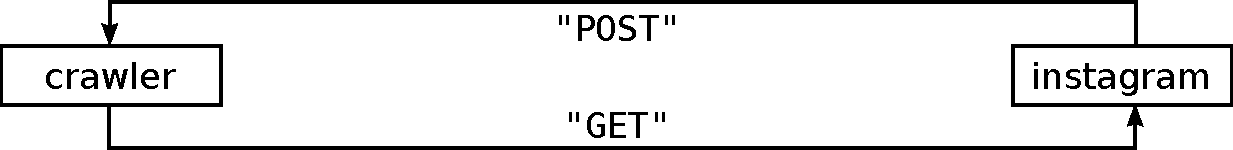
\includegraphics[width=\textwidth,keepaspectratio]{crawler.pdf}

	The response is a JSON file containing a list of media items. We save each of those items in a separate JSON file. We also save a thumbnail image for each media item.

	Our crawler is based on the software platform Node.js, which allows us to setup a http-server and request data in an asynchronous fashion with very little javascript code.
	\begin{quote}
		Node.js is a platform built on Chrome's JavaScript runtime. [..] It uses an event-driven, non-blocking I/O model that makes it lightweight and efficient, perfect for data-intensive real-time applications that run across distributed devices.\footnote{\url{http://nodejs.org/}}
	\end{quote}

	Instagram allowes developers to issue 5000 requests per hour\footnote{\url{http://instagram.com/developer/endpoints/}}, thus we introduced a politeness factor $p$: Only every $p$-th time our crawler is notified we actually request the new data. This has two effects: First, the number of requests is reduced and second, the number of new media items per response is higher. It also means that we probably miss a fraction of the data. However, if one would setup a larger system with multiple crawlers the coverage would increase.



\section{Indexing}
\end{document}
